\section{Methodology}

In this section, we outline the rationale for decentralization, introduces the DeQA mechanism with a tokenomics–knowledge dual loop, analyzes its game-theoretic guarantees under Nash equilibrium, and discusses the supporting decentralized technologies.
% We posit that modern internet applications are undergoing a profound paradigm shift toward user-centric, autonomous, and decentralized paradigms that challenge traditional centralized architectures. These emerging systems fundamentally challenge traditional centralized models by redistributing control over data, computation, and economic value. To support this claim, we focus on Decentralized Agentic Question Answering as a representative scenario and explore two complementary perspectives:

% $\bullet$ \textbf{Technical Decentralization.}\textit{ How can the decentralized architecture be implemented through decentralized data ledgers, verifiable computation, and programmable smart contracts, to enable transparent, trustless, and auditably autonomous execution?}

% $\bullet$ \textbf{Economic Incentives.} \textit{How can the token-based incentive mechanism be structured to align agent interests, reward meaningful contributions, and foster long-term sustainability in decentralized communities without centralized enforcement?}

% \begin{figure}[htbp]
% \centering
% \includegraphics[width=1\textwidth]{figures/Decision_Making.pdf}
% \caption{Decision Making}
% % \vspace{-0.3cm}
% \label{Decision_Making}
% \end{figure} 





\subsection{Ecosystem Motivation}
The rise of knowledge-intensive online platforms has revolutionized how people seek, share, and evaluate information. In conventional question answering (QA) platforms, users generally alternate between two fundamental roles: consumers, who initiate domain-specific queries, and producers, who provide answers. Let $\mathcal{U}$ denote the user set, where each user $u \in \mathcal{U}$ possesses distinct expertise and may assume either role during an interaction.

\begin{definition}{\textbf{(Consumer)}}\label{def:consumer} 
A consumer $c \in \mathcal{U}$ issues a set of domain-specific queries $\mathcal{Q} = \{q_1, \cdots ,q_{N}\}$ and seeks to subscribe to a qualified producer $p \in \mathcal{U}$. For long-term service within the same domain, the consumer $c$ commits tokens for future interactions.
\end{definition}

\begin{definition}{\textbf{(Producer)}}\label{def:producer} 
A producer $p \in \mathcal{U}$ leverages their domain knowledge to generate responses $\mathcal{R}$ tailored to consumer $c \in \mathcal{U}$. By delivering high-quality and professional responses, the producer $p$ earns the tokens from the consumer $c$.
\end{definition}

To support large-scale knowledge exchange, centralized platforms monopolize the underlying infrastructure by dictating how data is stored, how algorithms are deployed, and how decisions are executed. More critically, they maintain total dominance over consumer-producer interactions by content moderation, query routing, and reward allocation. Nevertheless, such architectures pose inherent risks rooted in black-box operations and constrained user autonomy. This motivates to imagine a decentralized paradigm for the question-answering community. Within this paradigm, the central challenge turns to motivating users act honestly, rationally, and cooperatively across diverse tasks. This, in return, leads to a deeper question:
\textit{\textbf{What incentive mechanisms can encourage truthful contributions, align individual interests, and ultimately sustain long-term evolution of the ecosystem without centralized enforcement?}}

To overcome these limitations, our work presents a decentralized QA framework that embeds token-aligned incentive mechanisms and can be operated atop blockchain-based infrastructure. The design draws inspiration from Web3 systems, where validators serve as a trustless backbone by verifying transactions, maintaining consensus, and enforcing protocol-level rules, thereby securing system integrity without centralized authority. Building on this foundation, DeQA reconceptualizes validators from transactional verifiers to semantic routers, who are purposefully selected to leverage their domain knowledge to assess the alignment between a consumer’s query and a producer’s response. As a result, this transformation shifts their role from enforcing syntactic correctness to providing knowledge-intensive service on query–responder routing, which replaces centralized pipelines with transparent, auditable, and self-forcing resolution.

\begin{definition}{\textbf{(Validator)}}\label{def:validator} 
A validator $v \in \mathcal{U}$ is an independent participant who, upon request, leverages domain knowledge to evaluate the routing between a query $q \in \mathcal{Q}$ and a producer $p \in \mathcal{U}$. The validator’s role is to assess whether the producer can accurately and reliably address queries within the corresponding domain.
\end{definition}

\begin{figure*}[!tbp]
\centering
\vspace{-4mm}
\caption{Overall Promotion Workflow.
(1) A consumer broadcasts a sample query when an information need arises.
(2) A producer provides their answer and requests validators to assess its correctness.
(3) Validators independently generate answers, form a consensus, and return it to the producer.
(4) If the producer’s answer agrees with the consensus, the service capability is confirmed, and the producer proceeds with the promotion offer to the consumer.}
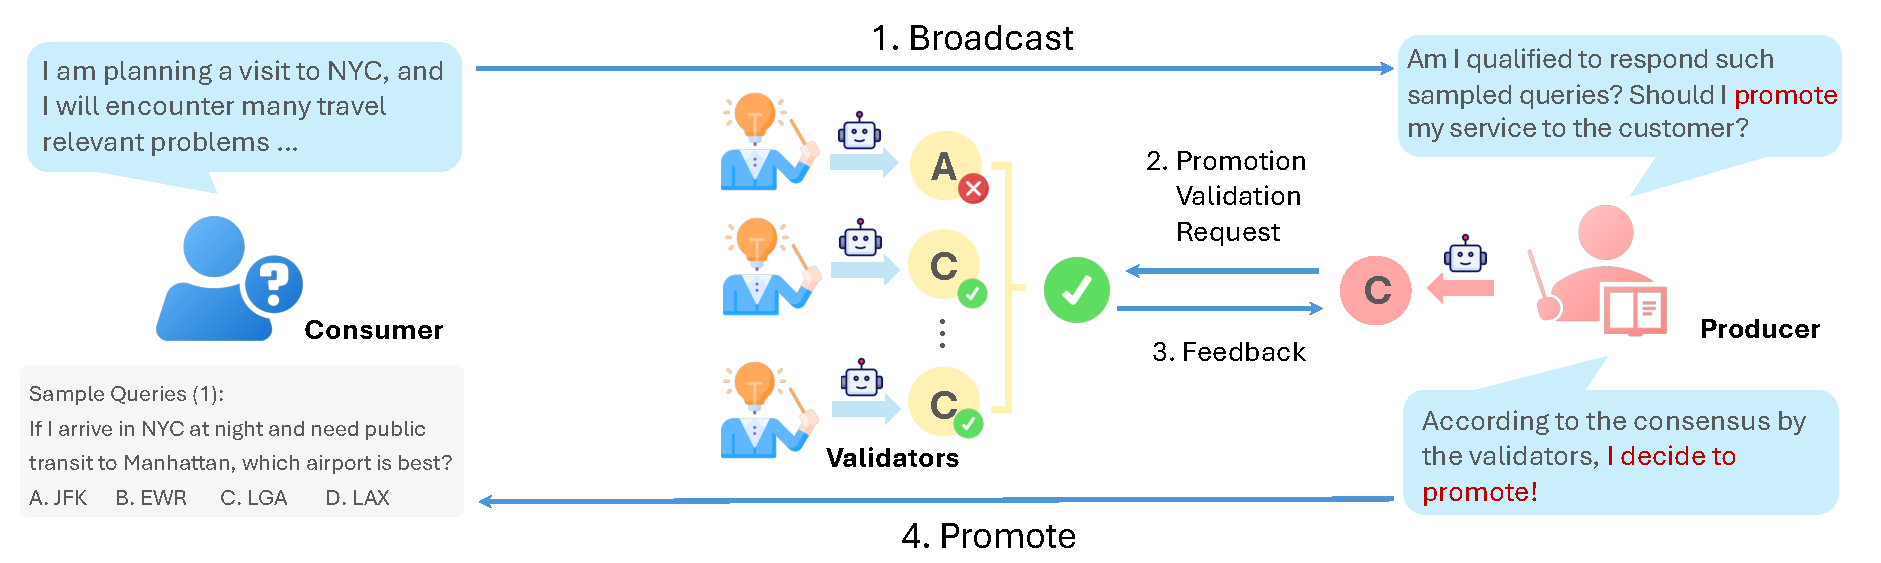
\includegraphics[width=\textwidth]{figures/Promotion.pdf}
\label{Promotion}
\vspace{-4mm}
\end{figure*} 

As their responsibilities evolve, validators emerge as indispensable participants in our decentralized ecosystem. They play a dual role: (i) economically, by reinforcing closed-loop incentive mechanisms (Section ~\ref{Tokenomics Incentives} and ~\ref{Game-Theoretic Guarantees}); and (ii) technically, by enabling auditable decentralized query-responder routing (Section ~\ref{Decentralization Techniques}).

\subsection{Mechanism Design}
\label{Tokenomics Incentives}

As shown in Figure \ref{Tokenomics}, each user can dynamically assume the roles of producer, consumer, or validator, engaging in activities such as posting queries, providing answers, and validating query–responder routing. Each role is incentivized through token-based rewards that align individual interests with the ecosystem's collective utility. Every action, whether promotion, subscription, or validation, not only contributes to knowledge exchange but also generate token flow, reinforcing sustainability and self-organization of the ecosystem.

\subsubsection{Promotion and Subscription}

The core structure of DeQA remains bounded to the conventional query–response–reward loop. Consumers post token-incentivized queries, while producers solve them to earn subscriptions in return, involving producer-initiated promotion and consumer-initiated subscription. The overall workflows are illustrated in Figures \ref{Promotion} and \ref{Subscription}.

\begin{definition}{\textbf{(Knowledge-intensive Service)}}\label{def:knowledge-intensive agent} 
Each user $u \in \mathcal{U}$ leverages personal domain knowledge $\mathcal{K}_u$ to provide a knowledge-intensive service $a_u: \mathcal{Q} \rightarrow \mathcal{R}$, whose quality level $q$ reflects the probability of generating correct responses, with a cost $c_u$ per call.
\end{definition}

Conceptually, $a_u$ is a non-transferable intellectual asset, permanently bound to its creator and analogous to a Non-Fungible Token (NFT) in Web3. Producers promote their services to attract subscriptions, while consumers subscribe to preferred producers for long-term knowledge support, creating a two-sided market.

$\bullet$ \textbf{Promotion.} 
When a consumer $c$ raises an information need with sample queries, a \underline{producer} $p$ may proactively promote their service $a_p$ to attract potential subscription. To initiate this promotion, the producer pays a token fee $\tau_p$ to broadcast their availability.

$\bullet$ \textbf{Subscription.}
After reviewing promotions, the \underline{consumer} $c$ may subscribe to the preferred producer’s service $a_p$. By paying a subscription fee $\tau_s$ in tokens, the consumer delegates future problem-solving to $a_p$ and gains access to its ongoing services.

In practice, promotion and subscription are high-stakes, long-term commitments with substantial token expenditure. Poor matches not only erode user trust but also undermine incentive alignment. Therefore, accurate and truthful query–responder routing is critical for maximizing utility and ensuring efficient token allocation. 


\subsubsection{Validation Requests }


In conventional QA, query–responder routing relies heavily on subjective judgments. Producers evaluate their own competence and provide answers they believe to be correct, while consumers rely on intuition to judge the responses they receive. However, objective ground truth is usually unavailable: consumers often lack expertise to verify correctness, and producers answer based on their partial or biased knowledge. This asymmetry between knowledge supply and demand frequently leads to suboptimal and unreliable routing outcomes.

% In conventional QA scenarios, query-responder routing primarily depends on the producer's self assessment and the consumer’s intuitive judgment. However, in many cases, no objective ground truth is available. Producers may be uncertain about the correctness of their responses, while consumers naturally lack the domain expertise needed to assess agent competence.
% This mismatch between knowledge supply and demand, rooted in information asymmetry and bounded rationality, frequently leads to suboptimal or unreliable routing decisions.

To address this issue, heterogeneous third-party validators make independent decision and reach consensus, yielding outcomes that should be more objective and reliable. Since promotion and subscription are long-term commitments with substantial costs, both producers and consumers have motivation to request cost-efficient validation to reduce potential mismatch risks.

$\bullet$ \textbf{Promotion Validation Request.} When a consumer $c$ raises an information need with a sample query set $\mathcal{Q}_{c} \subset \mathcal{Q}$, the \underline{producer} $p$ requests validation from a group of validators $V_p \subset \mathcal{U}$ before initiating a formal promotion, where $|\mathcal{Q}_{c}| = m$ and $|V_p| = n$. 
Each validator receives a fixed validation fee $\tau_{\text{val}}$ for one query, paid by the producer, where $m \times n \times \tau_{\text{val}} \ll \tau_p$ and $c_u < \tau_{\text{val}}$.

$\bullet$ \textbf{Subscription Validation Request.}
When a consumer $c$ receives promotions from multiple producers and needs to choose a preferred one, the \underline{consumer} issues another query set $\mathcal{Q}_s \subset \mathcal{Q}$ to disjoint validators ${V}_s \subset \mathcal{U}$, where $|\mathcal{Q}_{s}|= m$ and $|V_s| = n$. Note $\mathcal{Q}_s \cap \mathcal{Q}_p = \varnothing$ and ${V}_s \cap {V}_p = \varnothing$. 
Each validator will be compensated with the same fee $\tau_{\text{val}}$ for a call, paid by the consumer, where $m \times n \times \tau_{\text{val}} \ll \tau_p$ and $c_u < \tau_{\text{val}}$.

Validators harness their knowledge to provide decentralized decisions, and the requester considers their consensus as a reference.


\begin{figure*}[!htbp]
\centering
% \vspace{-5mm}
\caption{Overall Subscription Workflow.
(1) Upon receiving a promotion, the consumer issues new sample queries and requests fresh validators to assess the producer’s capability.
(2) Validators independently generate their answers and reach a consensus.
(3) The producer responds with its own answer to the same query.
(4) Validators return the consensus result.
(5) The consumer compares the two answers and decides whether to subscribe to the service for future queries.}
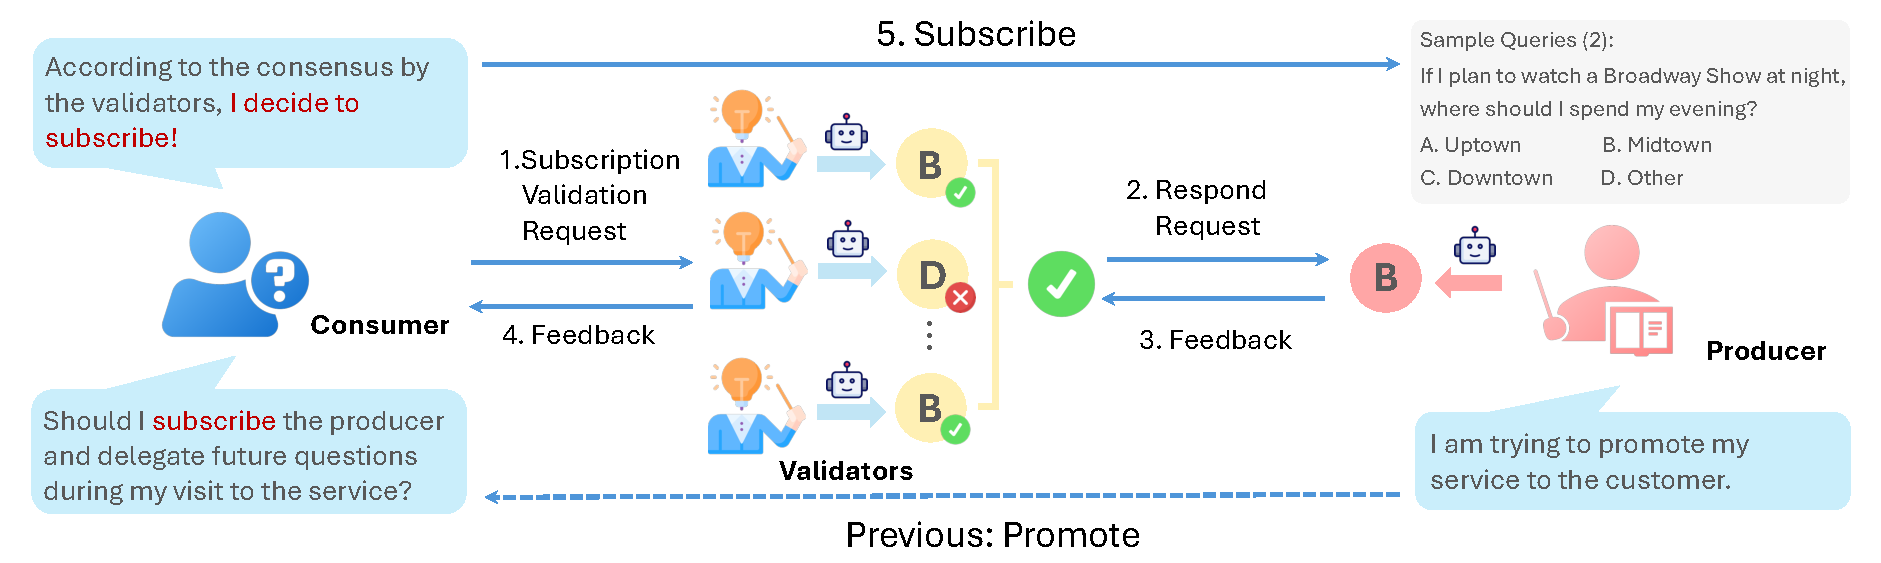
\includegraphics[width=\textwidth]{figures/Subscription.pdf}
% \vspace{-4mm}
\label{Subscription}
\end{figure*} 


\subsubsection{Validation Workflow}
We employ a tokenomics-driven decentralized validation mechanism in which heterogeneous validators collaborate to deliver more convincing consensus, aiming to improve the transparency and auditability of query–responder routing.
Upon request, selected validators serve as a decentralized proxy to assess query–responder alignment by checking whether the validator's answer concurs with the responder’s answer. These assessments are aggregated through majority voting to form a consensus, which is then returned to the requester, either the producer (in promotion validation) or the consumer (in subscription validation), as a reference for final routing decisions.

$\bullet$ \textbf{Vote for Consensus in Promotion.}
Let $V_p = \{ v_1, \cdots, v_n \}$ with $n \ll N$ denote the validators involved in promotion validation. Each validator $v_i \in V_p$ independently produces a judgment $r_i = a_i(\mathcal{Q}_p, a_p)$ by comparing its own answers with those generated by the candidate service $a_p$ on the sample query set $\mathcal{Q}_p$. A consensus $r^*$ is then derived through majority voting:
\begin{equation}
r^* = \text{MajorityVote}\left( \{ r_1, \dots, r_n \} \right).
\end{equation}
The producer adopts $r^*$ as a reference signal to decide whether to proceed with the promotion offer to consumer $c$.

% Assume $V_P=\{ v_1, \dots, v_n\}$, Each validator $v_i\in V_P$ independently generates a response $r_i$ using their agent, and a consensus $r^*$ response is computed via majority voting:
% \begin{equation}
%     r^* = \text{MajorityVote}\left( \left\{ r_1, \cdots, r_n\right\} \right).
% \end{equation}
% The producer compares $r^*$ with their own agent output $r_p$ to decide whether to proceed with promotion. 

$\bullet$ \textbf{Vote for Consensus in Subscription.}
Similarly, let $V_s = \{ v_1', \dots, v_n' \}$ with $n \ll N$ denote the validators selected for subscription validation. Each validator $v_j \in V_s$ compares its own answers with those from the producer’s service $a_p$ on a separate query set $\mathcal{Q}_s$, and outputs a local judgment $r_j' = a_j(\mathcal{Q}_s, a_p)$. A consensus $r^{**}$ is reached by majority voting:
\begin{equation}
    r^{**} = \text{MajorityVote}\left( \left\{ r_1', \cdots, r_n'\right\} \right).
\end{equation}
The consumer uses $r^{**}$ to decide whether $a_p$ is sufficiently aligned with their domain expectations and worthy of subscription.

The requester may either accept or reject the consensus and make the final decision.
Once a subscription is confirmed, the producer becomes obligated to respond to future queries under a token-backed commitment, which can be enforced through smart contracts. We highlight several key design principles as follows.

$\bullet${\textbf{ Proof-of-Intelligence (PoI).}}\label{poi}
We introduce a validation mechanism called Proof-of-Intelligence (PoI),  inspired by Proof-of-Work (PoW)\cite{jakobsson1999proofs} and Proof-of-Stake (PoS)\cite{dwork1992pricing} in blockchain. Unlike PoW and PoS, which rely on computational power or financial resources, PoI is grounded in \textit{domain-specific knowledge} and \textit{verifiable intellectual efforts} contributed by human validators. In this way, PoI operationalizes epistemic labor as a stakeable and rewardable asset for decentralized coordination.

$\bullet$ {\textbf{Knowledge as Monetization Tool.}}
The knowledge-intensive service embodies a producer’s intellectual capability and serves as the monetization interface in transactions, either by being subscribed or participating in validation. In this way, the system incentivizes producers to continuously refine high-quality service and delivering reliable outcomes.

\subsubsection{Rewards and Penalties in Validation.}

It is worth highlighting that, unlike platform-curated matching, validator consensus dynamically reflects collective domain judgments. This design fosters epistemic pluralism, enabling knowledge discovery even under ambiguous or ill-defined query contexts. Nevertheless, the effectiveness of decentralized validation hinges on incentive-compatible mechanisms that, by design, induce participants to act truthfully and cooperate out of rational self-interest.

$\bullet$ \textbf{Tokenomics in Validation.} To participate in validation, each validator must stake a fixed amount of tokens $\sigma$ as a cost commitment, creating financial exposure to deter dishonest behavior. Once voting concludes, a validator is rewarded if its local judgment aligns with the consensus, i.e., $r_i = r^*$ in promotion or $r_j' = r^{**}$ in subscription. Rewards come from both the requester’s payment ($M \times n \times \tau_{\text{val}}$) and a shared reward pool contributed by all participating validators themselves ($n\sigma$). Validators who deviate from the consensus forfeit their stake and receive no reward. All payments and staking operations are executed via smart contracts to ensure transparency, verifiability, and tamper-resistance. 

$\bullet$ \textbf{Moral Hazard in Validation.} We note that validators may not always participate honestly in the validation process. When exerting effort and reporting truthfully, a validator produces an evaluation of quality $q$ at a cost $c_u$; however, by shirking, they can generate a random judgment at no cost. This contrast highlights the need for incentive constraints in validation, which will be elaborated in Section ~\ref{Incentive Compatibility of Validators}.

$\bullet$ \textbf{Utility-based Acceptance after Validation.} Meanwhile, the requester does not necessarily accept the consensus outcome, as their decision depends on their utility function and individual tolerance for service quality. Based on individual rationality, there exists a threshold at which producers or consumers decide whether to adopt the validation consensus. which will be further investigated in Section~\ref{Producer's Threshold-Optimal Promotion} and ~\ref{Consumer's Threshold-Optimal Subscription}.


% $\bullet${\textbf{ Fault Tolerance via Incentive and Game-Theoretic Design.}}
% Given the open nature of decentralized participation, we make no assumption of perfect validator behavior. Instead, reliability is enforced via an incentive-compatible design: validators are rewarded for aligning with consensus and penalized otherwise.
% First, occasional validator errors are tolerated under the Byzantine fault-tolerant (BFT) assumption, as long as a majority of validators remain honest and competent. Second, because validators make decisions independently, the system forms a decentralized game-theoretic structure resembling a prisoner's dilemma, which discourages collusion and reduces strategic dependency.

The advantages of the validation process for the entire ecosystem are twofold.
Economically, validators contribute intellectual effort and are compensated with tokens, reaffirming that knowledge possesses intrinsic and exchangeable economic value.
Technically, decentralized consensus mitigates centralized manipulation and promotes transparent, democratic coordination.



\subsubsection{Ecosystem Overview.}
We have observed that tokenomics is the primary driving force behind the prosperity of our decentralized ecosystem.
Table~\ref{tab: token flow} summarizes the token flow across roles and actions, illustrating how individual behaviors are linked to quantifiable incentives and how role coordination emerges organically without centralized orchestration. 

$\bullet$ \textbf{Mechanism Design.}
Our tokenomics framework incentivizes users to participate across different roles by coupling each role with both token-earning and token-spending opportunities. This knowledge-coordinated incentive mechanism forms a closed-loop economic loop, enabling a synergistic circulation of both knowledge and tokens as co-reinforcing resources.

$\bullet$ \textbf{System Implications.}
This ecosystem eliminates centralized control and supports protocol-level autonomy, through transparent and auditable rules rather than platform interventions. Role fluidity and action-value duality promote high-quality participation, foster decentralized coordination, and discourage manipulation, driving long-term sustainability and evolution.


% This tokenomics framework ensures incentive compatibility and strategic stability, motivating users to contribute across diverse roles and fostering long-term engagement within a self-sustaining community.


% \begin{table*}[!htbp]
% \centering
% \vspace{-5mm}
% \caption{Token flow matrix across different roles and actions. Regardless of roles, users earn tokens by contributing their agent services, while also spending tokens to access knowledge from others, even under asymmetric expertise.}
% \vspace{-2mm}
% % \resizebox{0.7\textwidth}{!}
% \setlength{\tabcolsep}{14pt}
% {
% \begin{tabular}{c|c|c|c|c}
% \midrule
% {Role} & {\makecell[c]{Promotion}} & {\makecell[c]{Subscription}} & {\makecell[c]{Promotion  Validation}} & {\makecell[c]{Subscription  Validation}} \\
% % \\
% \midrule
% Producer & {$-\tau_p$} & $+\tau_s$ & $-\tau_{val}$ & -  \\
% \midrule
% Consumer & $+\tau_p$ & $-\tau_s$ & -  & $-\tau_{val}$  \\
% \midrule
% Validator & - & -& \multicolumn{2}{l}{\makecell[l]{if agree with the consensus: $+(mn\tau_{val}+n\sigma)/n_{agree}$ \\ if disagree with the consensus: $-\sigma$}}  \\
% \midrule
% \end{tabular}
% }
% \vspace{-4mm}
% \label{tab: token flow}
% \end{table*}


\subsection{Game-Theoretic Guarantees for Incentives} 
\label{Game-Theoretic Guarantees}

In this section, we first establish validator incentive compatibility, ensuring that PoI voting truthfully aggregates dispersed knowledge. Building on this foundation, we derive threshold-optimal decision rules for consumer subscription and, subsequently, for producer promotion. Finally, by combining these IC and IR conditions, we demonstrate the existence of a symmetric Bayesian–Nash equilibrium (BNE) characterized by positive surplus, budget balance, and dual closed loops connecting tokens and knowledge.

% \subsubsection{Annotations and Assumptions.}
\subsubsection{Incentive Compatibility (IC) of Validators.} 
\label{Incentive Compatibility of Validators}

We formalize incentive compatibility (IC) for validators in the Bayesian validation game. Assume there are $n$ validators, where $n$ is odd. The requester pays each validator a fee $\tau_{\text{val}}$; each validator stakes \(\sigma\). If a validator’s report matches the majority, they obtain a conservative per-capita reward as $R_{\min}=\tau_{\text{val}}+\sigma$, otherwise they forfeit \(\sigma\).
Assume the other validators exert effort and report truthfully with individual quality $q_v$. Let $P_{\text{match}}(n,q_v)>\frac{1}{2}$
denote the probability that a truthful vote matches the majority, where tie-breaking under odd \(n\) is implicit. The expected truthful effort and free-riding (random vote) are: 
\[
\mathbb{E}[U\mid e{=}1]
= P_{\text{match}}\,R_{\min}-(1-P_{\text{match}})\sigma - c_u.
\]
\[
\mathbb{E}[U\mid e{=}0]
= \tfrac12\,(R_{\min}-\sigma).
\]

\begin{theorem}[IC Condition for Validators]
\label{Strict IC for Validators}
Validation is effective only if a validator’s expected payoff from truthful effort strictly exceeds that from free-riding. Thus, truthful effort is a strict best response iff

\[
% \boxed{(\text{IC}_{\text{exact}}) \quad 
(\tau_{val}  + 2\sigma)\Big(P_{\text{match}}(n,q_v) - \frac{1}{2}\Big) > c_u.
% }
\]
\end{theorem}

Only when this holds, does validation remain effective, delivering an incentive-compatible validation layer in the Bayesian game.
Larger \(\tau_{\text{val}}\) or \(\sigma\) strengthens incentives, and higher \(q_v\) or \(n\) and raise $P_{\text{match}}$, expanding the IC region for a global equilibrium.


\subsubsection{Producer's Threshold-Optimal Promotion}
\label{Producer's Threshold-Optimal Promotion}

We characterize the supply-side best response in our two-stage mechanism, seeking a threshold-based policy based on individual rationality. Assume a producer with quality $q_p$ pays a promotion fee $\tau_p$ and, if requesting promotion-time validation, pays each of the $n$ validators a fee $\tau_{\text{val}}$ for one call. Majority voting generates a public signal $Z\in\{0,1\}$ as consensus. Under the Monotone Likelihood Ratio Property (MLRP), the pass probability $V_p(q_p)=\Pr(Z=1\mid q_p)$ is strictly increasing in $q_p$.
Let $c_s>0$ be the net present value from a successful subscription from the consumer.
% . Given the need to pay validation fee and post-validation subscription prospects, we
% 
% , i.e. expected subscription revenue net of future service cost.

\begin{theorem}[IR-based Policy for Producers]
\label{Strict IC for Validators}
The optimal policy is a threshold rule for promotion that there exists $\bar q_p$ such that
\[
% \boxed{
\;V_p(q_p)\,(\tau_s - c_s )\;\ge\;\tau_p+mn\tau_{\text{val}}
\;\Longleftrightarrow\; q_p\;\ge\;\bar q_p\;.
% }
% \tag{TH--P}
\]

\end{theorem}
Hence, the promotion is the producer’s best response iff quality exceeds the threshold implied by costs and subscription prospects. 
This implements supply-side self-screening: only sufficiently competent producers rationally choose promote themselves.
% This aligns with validator IC (truthful effort) and consumer IR (subscription threshold), providing the supply-side component of a \textbf{symmetric Bayesian–Nash equilibrium} and improving routing efficiency without centralized curation.
Parameters steepening $V_p$ such as larger sampled query count or validator count could lower $\bar q_p$, whereas higher $\tau_p$ or $\tau_{\text{val}}$ raises it.


\subsubsection{Consumer's Threshold-Optimal Subscription.}
\label{Consumer's Threshold-Optimal Subscription}
Similarly, we provide the demand-side best response to decide when is it individually rational (IR) for a consumer to subscribe. The target is a threshold policy consistent with validator IC and the producer's entry rule.
The subscription fee is $\tau_s$. If subscription-time validation is requested, the consumer pays each of the $n$ validators a fee $\tau_{\text{val}}$.
Majority voting produces $Z\in\{0,1\}$.
Under MLRP, more favorable $Z$ implies a higher posterior utility value $\mathbb{E}[V_c(q_p)\mid Z]$, with $V_c(\cdot)$ strictly increasing in quality $q_p$.

\begin{theorem}[IR-based Policy for Consumers]
\label{IR-based Policy for Consumers}
The optimal policy is a threshold rule for subscription there exists $\bar q_c$ such that
\[
% \boxed{
\mathbb{E}[V(q_p)\mid Z]\;\ge\; \tau_s+mn\tau_{\text{val}} \iff q_c \ge \bar q_c.\,
% }
% \tag{TH--P}
\]

\end{theorem}

Thus, subscribing according to the consensus yields a positive expected payoff.
This condition defines demand-side IR screening: the consumer’s posterior utility must exceed a quality threshold before committing tokens to subscription. Beyond ensuring IR, this rule aligns the mechanism’s three layers. Validator IC ensures that $Z$ is informative; the consumer's threshold translates this information into disciplined demand; and, together with the producer’s entry rule, these best responses jointly form a symmetric three-side equilibrium.
In practice, IRs for producers and consumers enhance both welfare and explainability: acceptance decisions are based on an auditable posterior test rather than opaque platform heuristics.
Higher $\tau_s$ or $\tau_{\text{val}}$ increases $\bar q_c$, while parameters that enhance validation informativeness, such as larger validator count $n$, greater sample size $m$, or higher validator accuracy $q_v$, tend to lower it. When a parameter influences both information and cost (e.g., $n$), its net effect on $\bar q_c$ depends on the calibration.





\subsubsection{Symmetric BNE and Closed Loops}
We integrate the incentive and threshold conditions derived for all roles into a unified equilibrium perspective. 
Our goal is to show that when validator IC, producer IR, and consumer IR jointly hold, the decentralized validation mechanism admits a \textbf{Symmetric Bayesian-Nash Equilibrium (BNE)}, ensuring consistent strategic behavior and stable routing outcomes across roles.

\begin{theorem}[Symmetric Bayesian Nash Equilibrium]
\label{Symmetric Bayesian Nash Equilibrium}
If the following three groups of inequalities hold simultaneously:

\[
\underbrace{(\tau_{\text{val}}+2\sigma)\big(P_{\text{match}}(n,q_v)-\tfrac12\big) > c_u}_{\text{V-IC}},
\qquad
\underbrace{q_p \geq \bar q_p}_{\text{P-IR}},
\qquad
\underbrace{q_c \geq \bar q_c}_{\text{C-IR}}.
\]

then a symmetric BNE exists such that:
\begin{enumerate}
    \item Each validator exerts effort and votes truthfully (Sec \ref{Incentive Compatibility of Validators});
    \item Each producer promotes their service only when confident that its quality exceeds the competence threshold (Sec \ref{Producer's Threshold-Optimal Promotion}).
    \item Each consumer subscribes only when the posterior utility, conditional on the consensus, meets the expected value (Sec \ref{Consumer's Threshold-Optimal Subscription});
\end{enumerate}
\end{theorem}

When all three roles’ best responses coincide within the same parameter region, the system reaches a self-consistent equilibrium in which every participant earns a non-negative expected payoff consistent with their IC or IR conditions.

\subsubsection{Tokenomics–Knowledge Dual Loop.}
At equilibrium, all roles act rationally and consistently: validators exert effort and report truthfully, producers promote only when confident in their service quality, and consumers subscribe only when posterior utility meets expectations.
This mutual alignment closes the tokenomics–knowledge loop, where validators ensure credible information, producers signal competence, and consumers reward reliability.
Through this mechanism, token circulation incentivizes truthful behavior, while credible information, in turn, reinforces token value.
The resulting equilibrium transforms individual rationality into collective stability and enables incentive-compatible ecosystem without centralized enforcement.

\subsection{Decentralization Techniques}
\label{Decentralization Techniques}

Blockchain can serve as the foundational trust layer of decentralized systems.
To prevent data monopolies, it records protocol states, ownership, validator decisions, and finalized outcomes through network-wide consensus.
Rich content and service agents are stored off-chain but cryptographically linked to on-chain records, ensuring both verifiability and efficiency.
This hybrid architecture combines \textbf{on-chain trust with off-chain scalability} and guarantees user data sovereignty. 
Meanwhile, \textbf{smart contracts} govern validator voting, reward distribution, stake slashing, and role operations such as promotion and subscription, enforcing auditable PoI mechanism and tokenomics–knowledge dual loop. By encoding coordination logic into the protocol, DeQA eliminates centralized control and turns social trust into transparent, programmable accountability.



% In our DeQA ecosystem, blockchain serves as the foundational infrastructure for enabling trustless coordination among participants. We outline how core system components, including data storage, model deployment, and decision-making processes, are implemented in a verifiable and tamper-resistant manner.

% \subsubsection{Decentralized Data Ledger.}
% To overcome the limitations of centralized data monopolies, we adopt a hybrid architecture that combines on-chain integrity with off-chain scalability. On-chain data, confirmed through network-wide consensus, anchors trust in decentralized QA ecosystem.
% It maintains (i) protocol state, including token balances, staking status, and contract logic; (ii) ownership bindings, mapping users to agents and digital assets; (iii) validator decisions, ensuring auditable consensus formation; and (iv) finalized consensus outcomes, such as agent-task assignment.

% However, due to its cost and storage limitations, the blockchain layer is unsuitable for hosting large-scale or semantically rich content. 
% Off-chain data is stored outside the blockchain but remains cryptographically anchored to on-chain states for verifiability.
% It supports (i) content data, such as full questions, answers, and message logs; (ii) knowledge assets, including user corpora and agent models; and (iii) sensitive metadata, like identity proofs and behavioral traces, which require flexible access control and privacy guarantees.
% This hybrid design enhances scalability, supports seamless integration of external AI components (e.g., LLM-based agent models), and enables a verifiable transition toward user-controlled data sovereignty.


% \subsubsection{User-controlled Agent Models.}
% \label{User-controlled Agent Models}
% In practice, each agent is instantiated as a Retrieval-Augmented Generation (RAG) pipeline, composed of a user-curated knowledge corpus and an LLM-based generator. This architecture empowers users to externalize their expertise through a queryable and verifiable interface, allowing others to evaluate, subscribe to, or reward the agent based on its response quality.

% \begin{definition}{\textbf{(RAG-based Agent)}}\label{def:rag-based agent} 
% Each user $u \in \mathcal{U}$ encapsulates their knowledge $\mathcal{K}_u$ into a personalized agent $a_u: \mathcal{Q} \rightarrow \mathcal{R}$. The agent is instantiated as a RAG pipeline powered by LLMs. Specifically, given a query $q \in \mathcal{Q}$, the agent first retrieves relevant entries from the user-curated knowledge base $\mathcal{K}_u$, and then generates a context-aware response $r \in \mathcal{R}$ using the LLM conditioned on the retrieved content.
% \end{definition}

% \subsubsection{Smart Contract.}
% \label{Smart Contract}
% A smart contract is a self-executing program deployed on the blockchain that enforces predefined rules and automates interactions among untrusted parties. Functionally, it serves as a decentralized commitment mechanism, i.e. a tamper-proof, delay-resistant, and nondiscriminatory protocol for executing agreements without relying on trusted intermediaries.
% In our decentralized QA ecosystem, smart contracts orchestrate the full lifecycle of interactions across roles, including validator voting, reward allocation, stake slashing, and agent-level operations such as promotion, subscription, and service access.
% By embedding coordination logic directly into the protocol, smart contracts remove the need for centralized control. They make all system behaviors transparent, verifiable, and self-enforcing. Beyond automation, they also transform informal social contracts, such as trust, accountability, and reputation, into programmable system components that can be audited and reused.


\begin{figure*}[t]
    \centering
    \vspace{-6mm}
    \begin{subfigure}[b]{0.162\linewidth}
        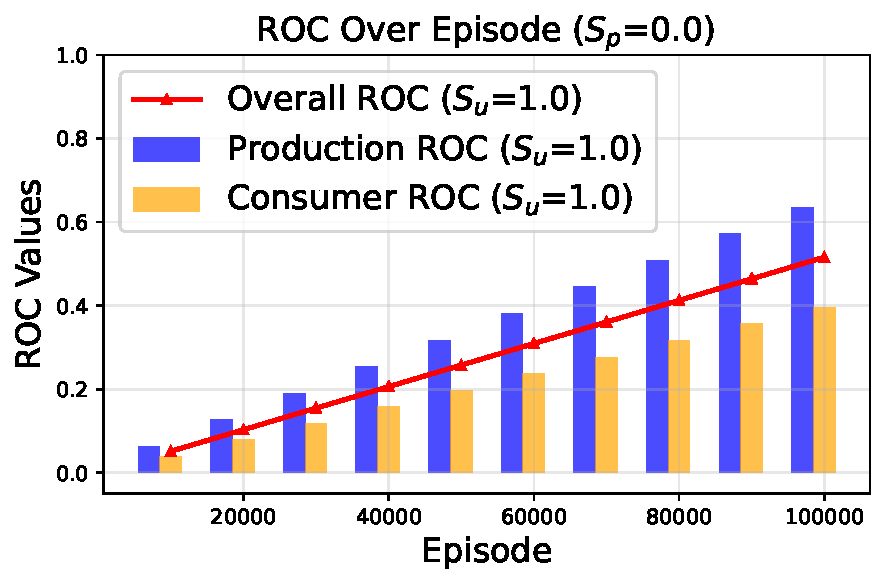
\includegraphics[width=\linewidth]{figures/fixed_sp/population_strategy_0_0_roc.pdf}
        % \caption{0}
    \end{subfigure}
    % \hfill
    \begin{subfigure}[b]{0.162\linewidth}
        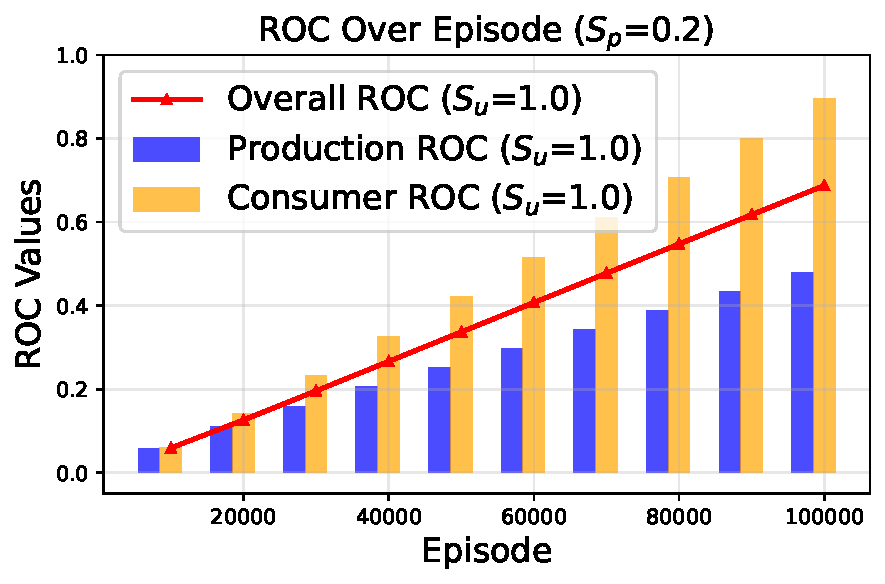
\includegraphics[width=\linewidth]{figures/fixed_sp/population_strategy_0_2_roc.pdf}
        % \caption{0.2}
    \end{subfigure}
    % \hfill
    \begin{subfigure}[b]{0.162\linewidth}
        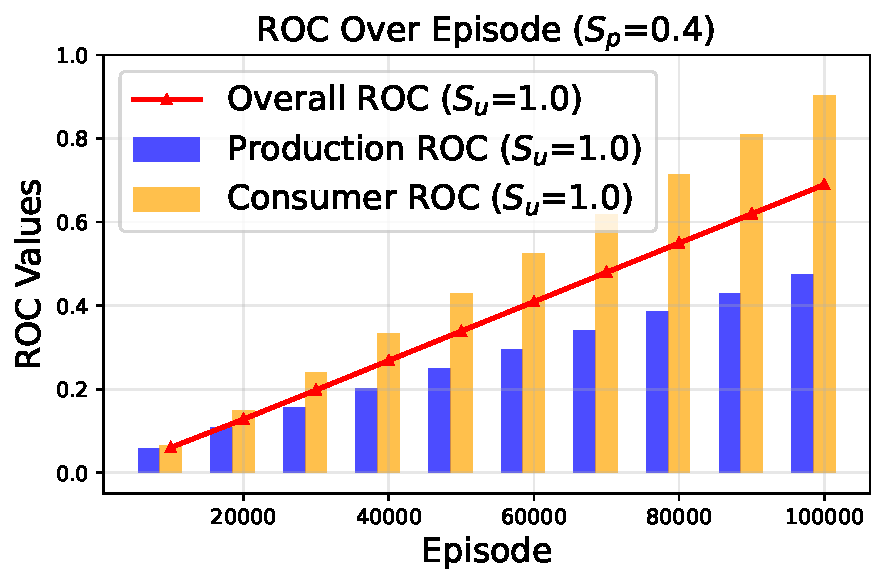
\includegraphics[width=\linewidth]{figures/fixed_sp/population_strategy_0_4_roc.pdf}
        % \caption{0.4}
    \end{subfigure}
    % \hfill
    \begin{subfigure}[b]{0.162\linewidth}
        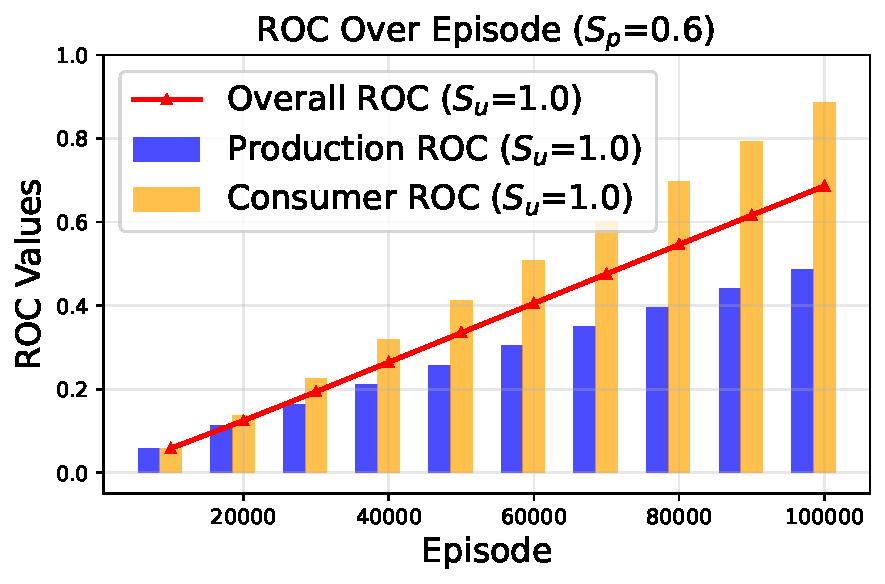
\includegraphics[width=\linewidth]{figures/fixed_sp/population_strategy_0_6_roc.pdf}
        % \caption{0.6}
    \end{subfigure}
    % \hfill
    \begin{subfigure}[b]{0.162\linewidth}
        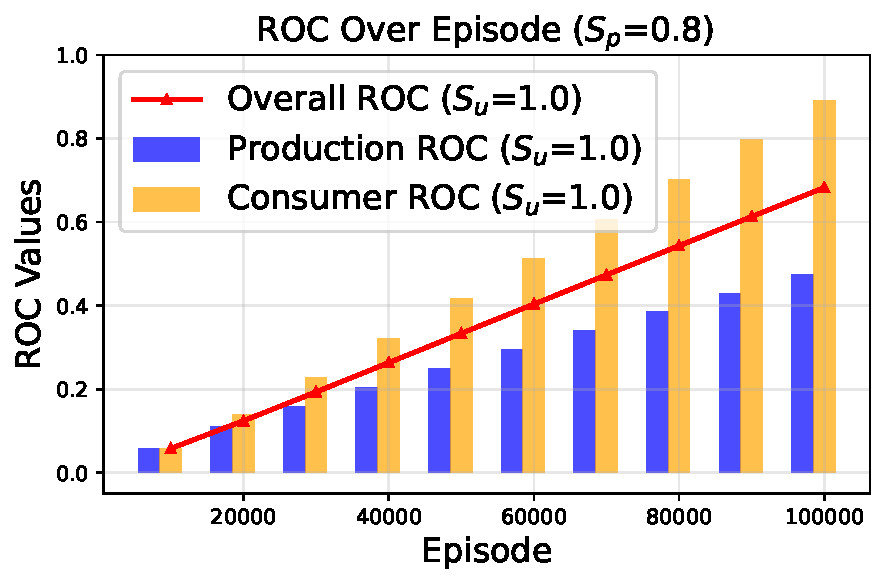
\includegraphics[width=\linewidth]{figures/fixed_sp/population_strategy_0_8_roc.pdf}
        % \caption{0.8}
    \end{subfigure}
    % \hfill
    \begin{subfigure}[b]{0.162\linewidth}
        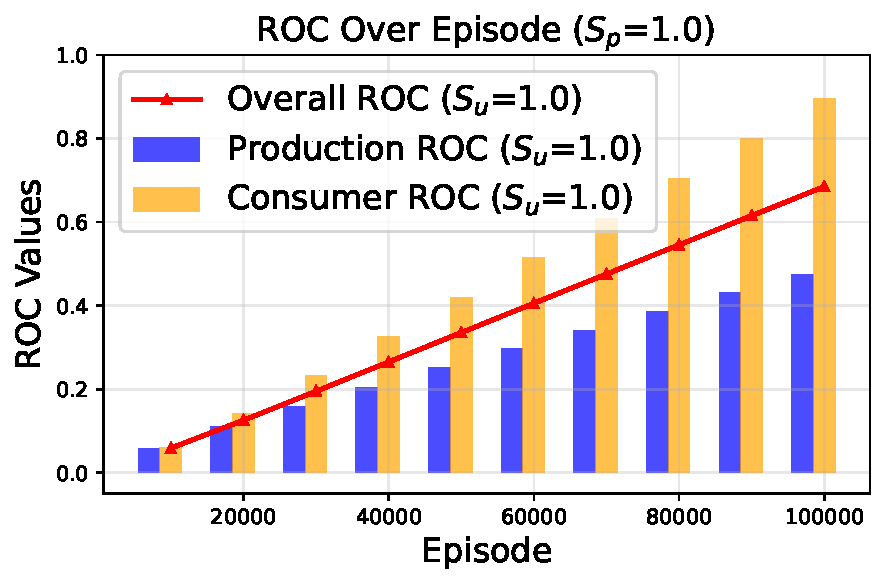
\includegraphics[width=\linewidth]{figures/fixed_sp/population_strategy_1_0_roc.pdf}
        % \caption{1.0}
    \end{subfigure}
    \vspace{1mm}
    \begin{subfigure}[b]{0.162\linewidth}
        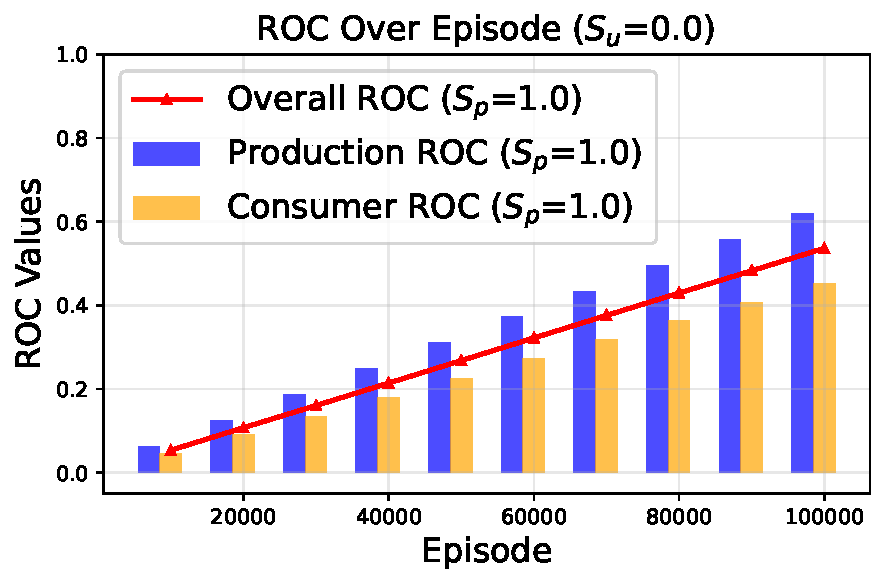
\includegraphics[width=\linewidth]{figures/fixed_su/user_strategy_0_0_roc.pdf}
        % \caption{0}
    \end{subfigure}
    % \hfill
    \begin{subfigure}[b]{0.162\linewidth}
        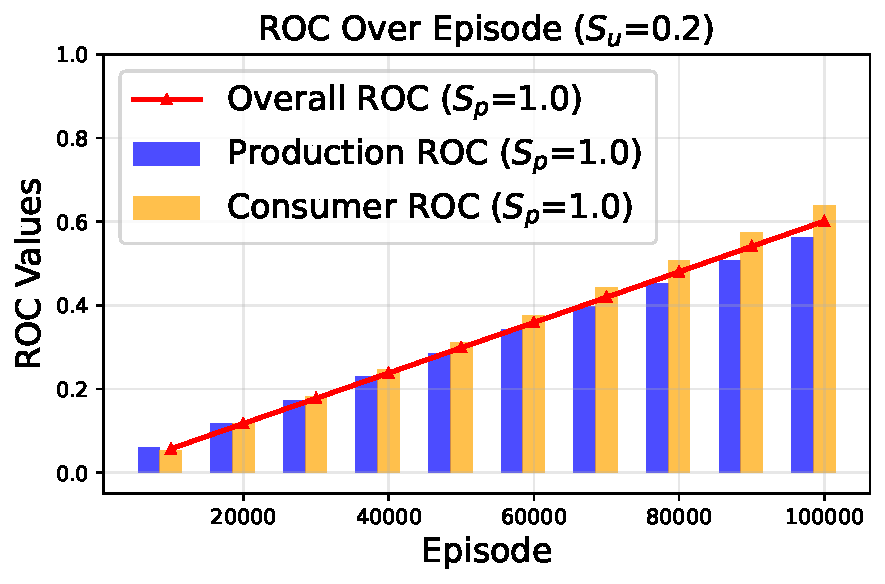
\includegraphics[width=\linewidth]{figures/fixed_su/user_strategy_0_2_roc.pdf}
        % \caption{0.2}
    \end{subfigure}
    % \hfill
    \begin{subfigure}[b]{0.162\linewidth}
        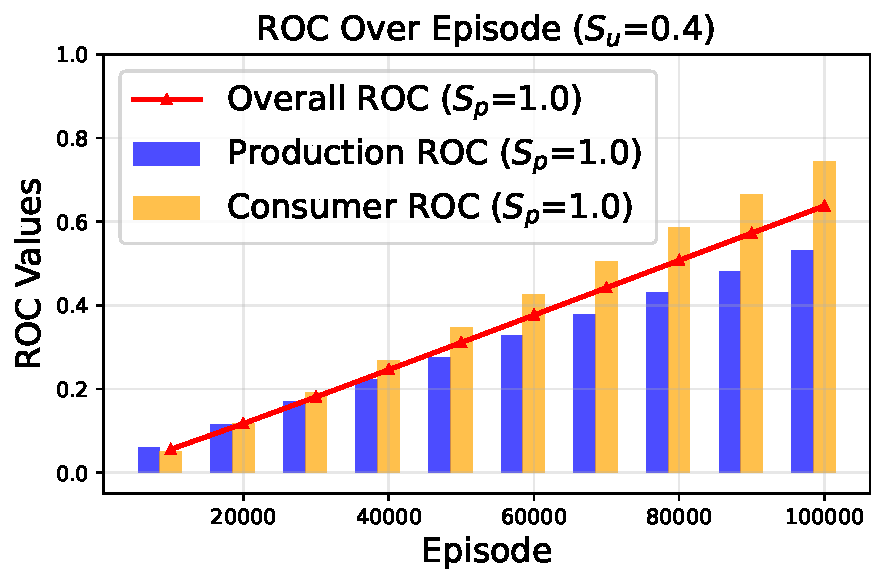
\includegraphics[width=\linewidth]{figures/fixed_su/user_strategy_0_4_roc.pdf}
        % \caption{0.4}
    \end{subfigure}
    % \hfill
    \begin{subfigure}[b]{0.162\linewidth}
        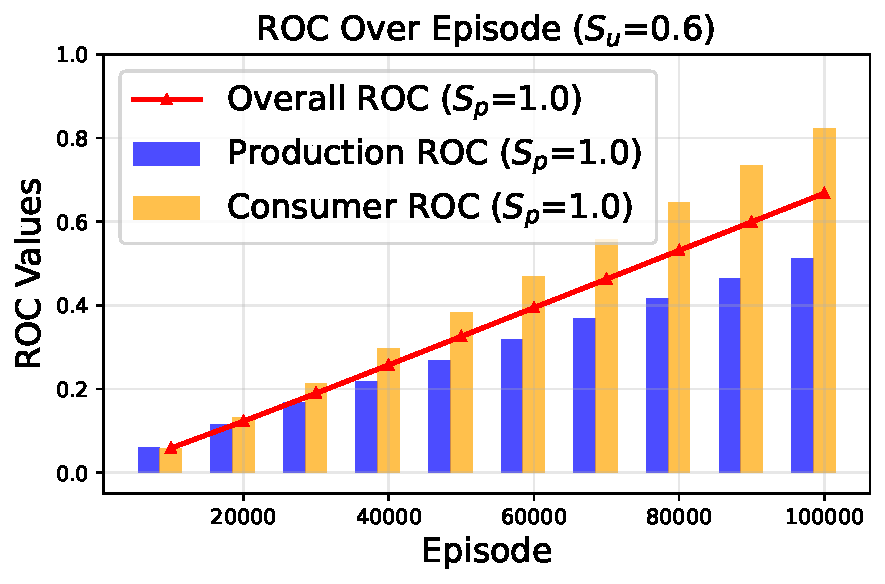
\includegraphics[width=\linewidth]{figures/fixed_su/user_strategy_0_6_roc.pdf}
        % \caption{0.6}
    \end{subfigure}
    % \hfill
    \begin{subfigure}[b]{0.162\linewidth}
        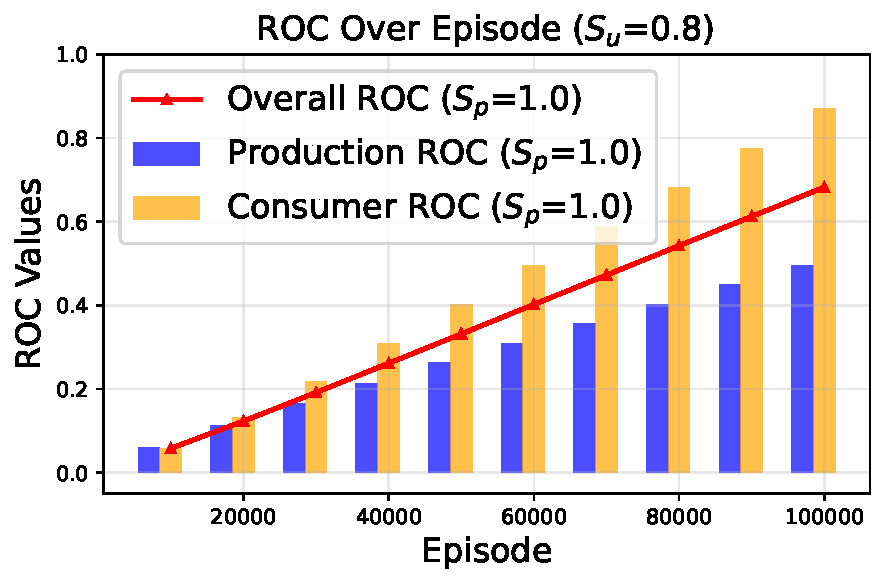
\includegraphics[width=\linewidth]{figures/fixed_su/user_strategy_0_8_roc.pdf}
        % \caption{0.8}
    \end{subfigure}
    % \hfill
    \begin{subfigure}[b]{0.162\linewidth}
        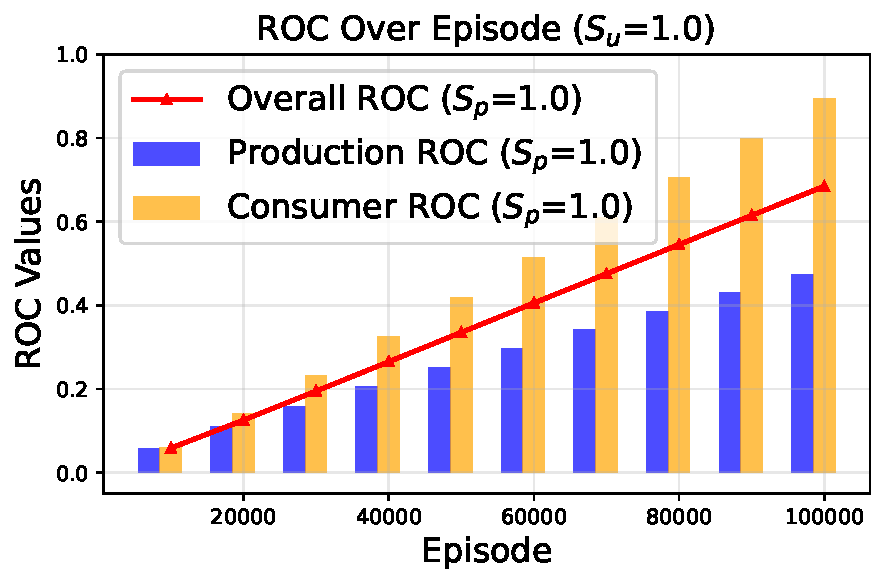
\includegraphics[width=\linewidth]{figures/fixed_su/user_strategy_1_0_roc.pdf}
        % \caption{1.0}
    \end{subfigure}
    \vspace{-4mm}
    \caption{ROC comparison over 100,000 episode based on different strategy. }
    \label{ROC Comp}
    \vspace{-1mm}
\end{figure*}

\begin{figure*}[t]
    \centering
    \begin{subfigure}[b]{0.162\linewidth}
        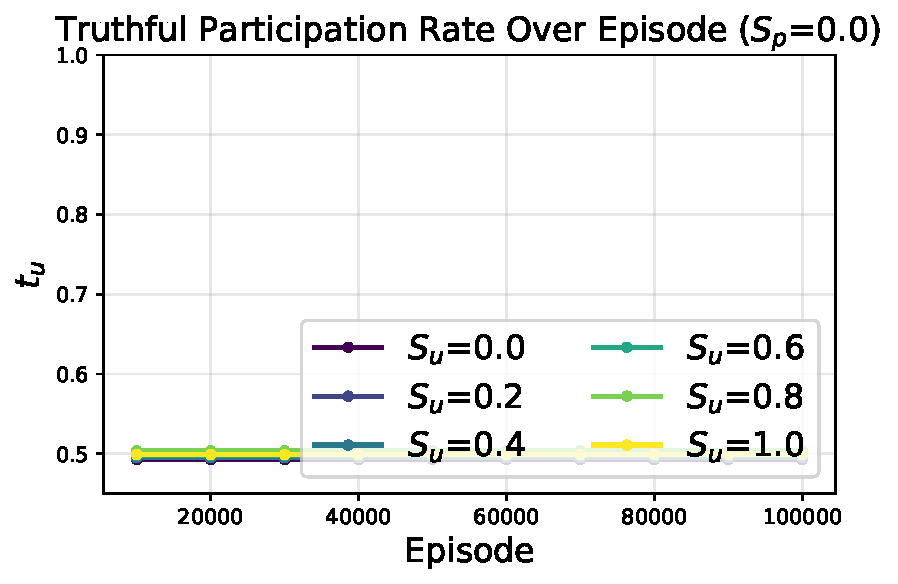
\includegraphics[width=\linewidth]{figures/fixed_sp/population_strategy_0_0_hard.pdf}
        % \caption{0}
    \end{subfigure}
    % \hfill
    \begin{subfigure}[b]{0.162\linewidth}
        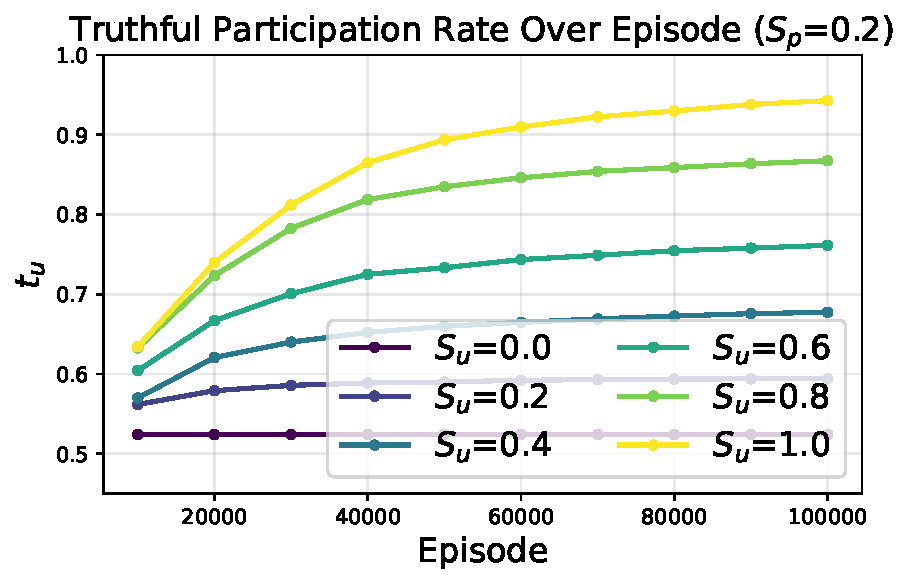
\includegraphics[width=\linewidth]{figures/fixed_sp/population_strategy_0_2_hard.pdf}
        % \caption{0.2}
    \end{subfigure}
    % \hfill
    \begin{subfigure}[b]{0.162\linewidth}
        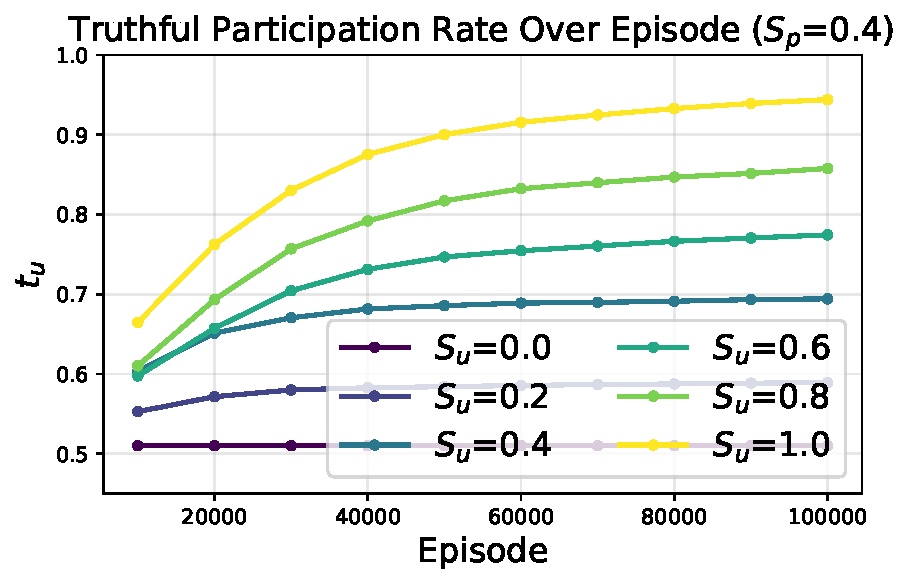
\includegraphics[width=\linewidth]{figures/fixed_sp/population_strategy_0_4_hard.pdf}
        % \caption{0.4}
    \end{subfigure}
    % \hfill
    \begin{subfigure}[b]{0.162\linewidth}
        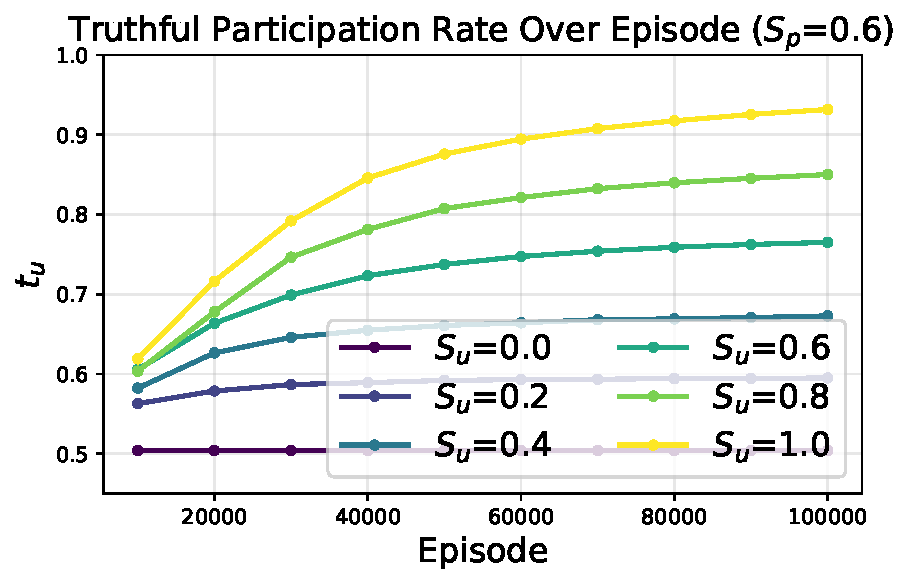
\includegraphics[width=\linewidth]{figures/fixed_sp/population_strategy_0_6_hard.pdf}
        % \caption{0.6}
    \end{subfigure}
    % \hfill
    \begin{subfigure}[b]{0.162\linewidth}
        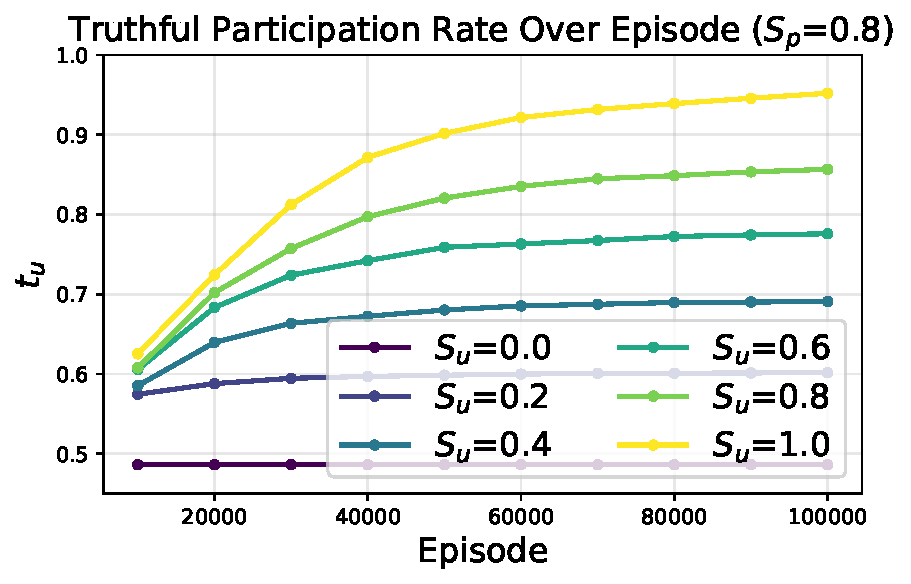
\includegraphics[width=\linewidth]{figures/fixed_sp/population_strategy_0_8_hard.pdf}
        % \caption{0.8}
    \end{subfigure}
    % \hfill
    \begin{subfigure}[b]{0.162\linewidth}
        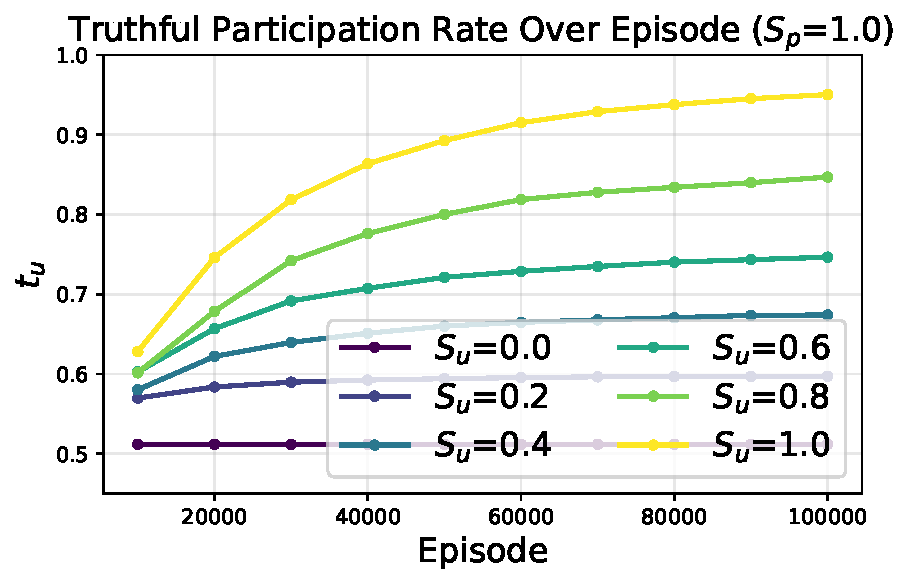
\includegraphics[width=\linewidth]{figures/fixed_sp/population_strategy_1_0_hard.pdf}
        % \caption{1.0}
    \end{subfigure}

    \vspace{1mm}

    \begin{subfigure}[b]{0.162\linewidth}
        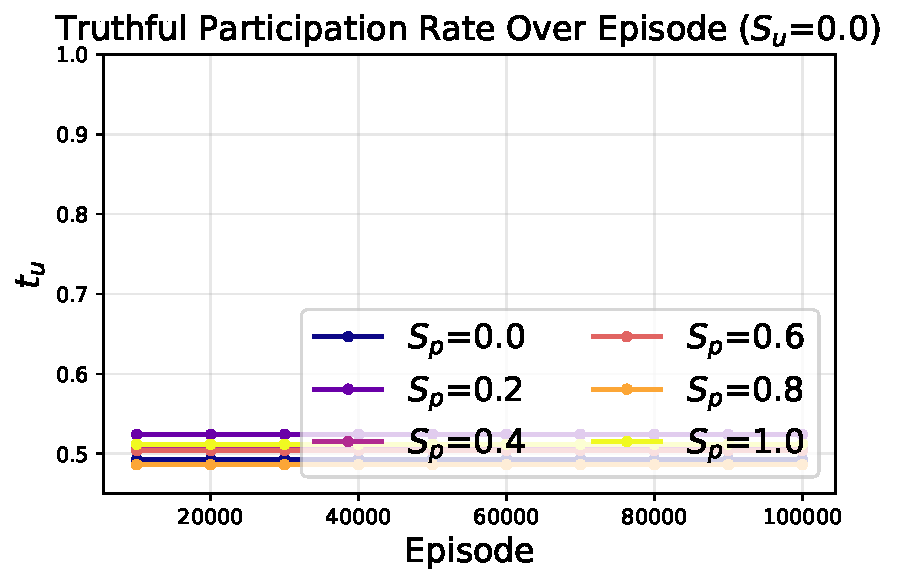
\includegraphics[width=\linewidth]{figures/fixed_su/user_strategy_0_0_hard.pdf}
        % \caption{0}
    \end{subfigure}
    % \hfill
    \begin{subfigure}[b]{0.162\linewidth}
        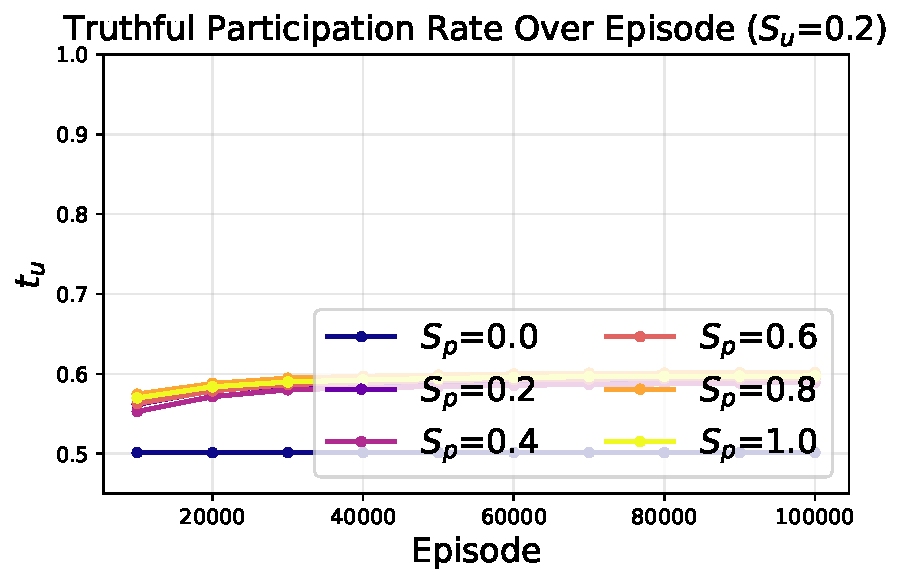
\includegraphics[width=\linewidth]{figures/fixed_su/user_strategy_0_2_hard.pdf}
        % \caption{0.2}
    \end{subfigure}
    % \hfill
    \begin{subfigure}[b]{0.162\linewidth}
        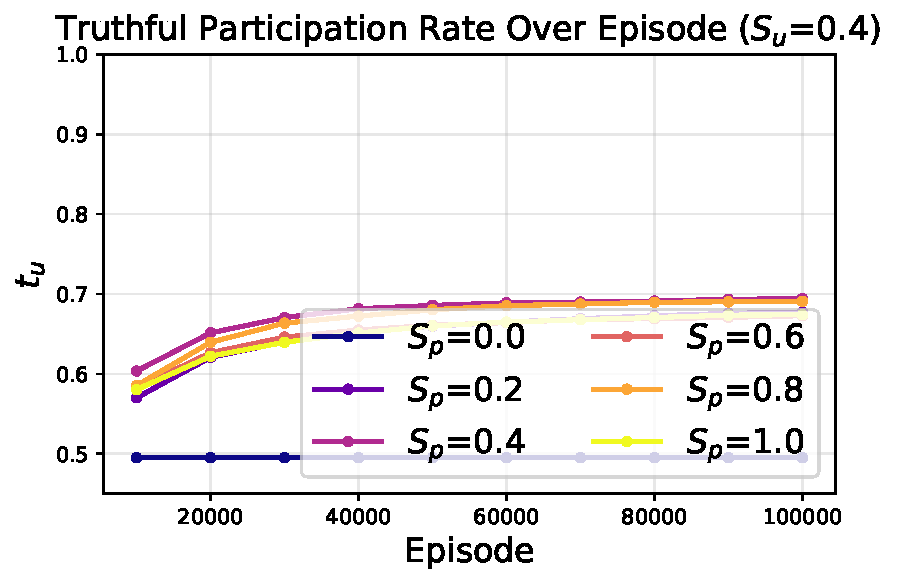
\includegraphics[width=\linewidth]{figures/fixed_su/user_strategy_0_4_hard.pdf}
        % \caption{0.4}
    \end{subfigure}
    % \hfill
    \begin{subfigure}[b]{0.162\linewidth}
        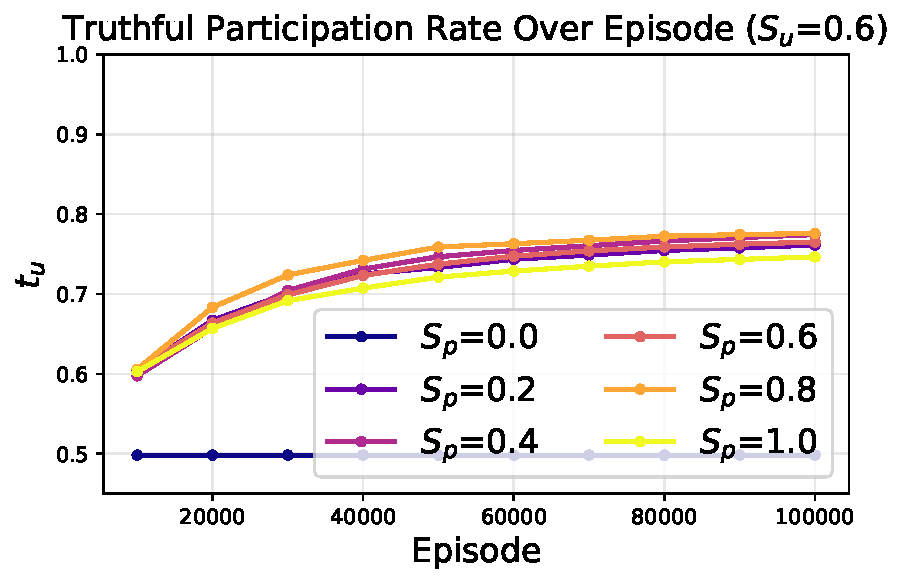
\includegraphics[width=\linewidth]{figures/fixed_su/user_strategy_0_6_hard.pdf}
        % \caption{0.6}
    \end{subfigure}
    % \hfill
    \begin{subfigure}[b]{0.162\linewidth}
        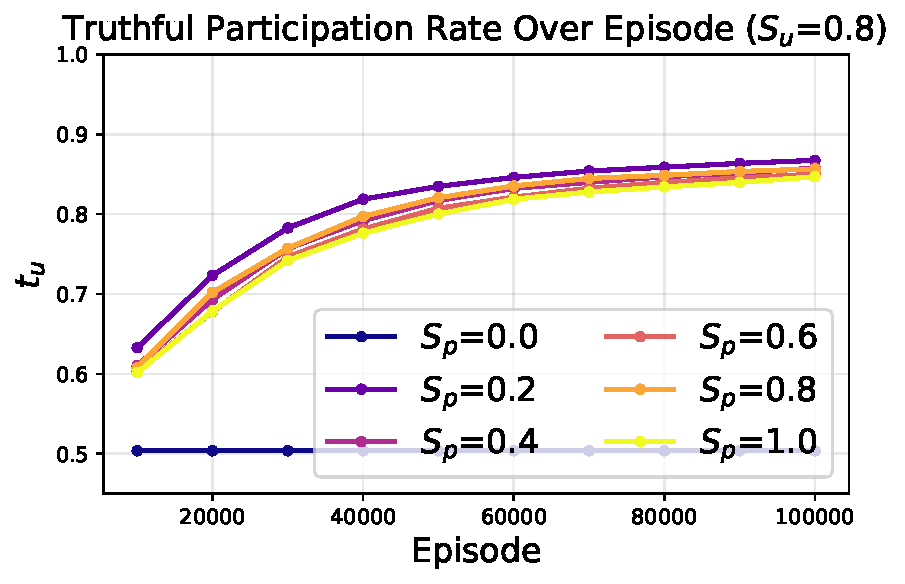
\includegraphics[width=\linewidth]{figures/fixed_su/user_strategy_0_8_hard.pdf}
        % \caption{0.8}
    \end{subfigure}
    % \hfill
    \begin{subfigure}[b]{0.162\linewidth}
        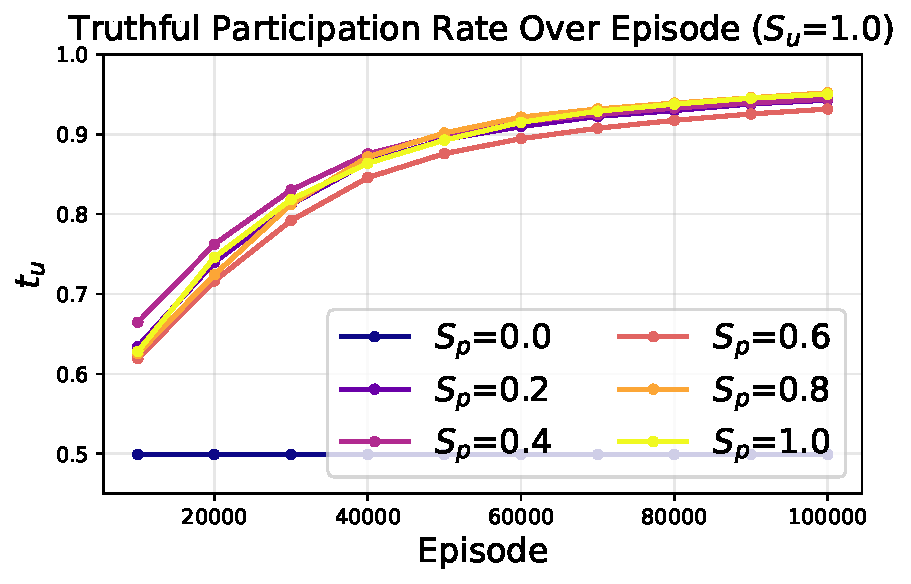
\includegraphics[width=\linewidth]{figures/fixed_su/user_strategy_1_0_hard.pdf}
        % \caption{1.0}
    \end{subfigure}
    \vspace{-3mm}
    \caption{Truthful participation comparison with different $S_{u}$ and $S_{p}$.}
        \label{Truthful participation comparison}
\end{figure*}
\vspace{-4mm}
